\begin{mainquestion}{curramp}{Current Amplifier Design}
The input of a current amplifier is to be connected to a current source with a source resistance $R_{s}$, and its output is connected to a load $R_{L}$, as shown below:

\begin{center}
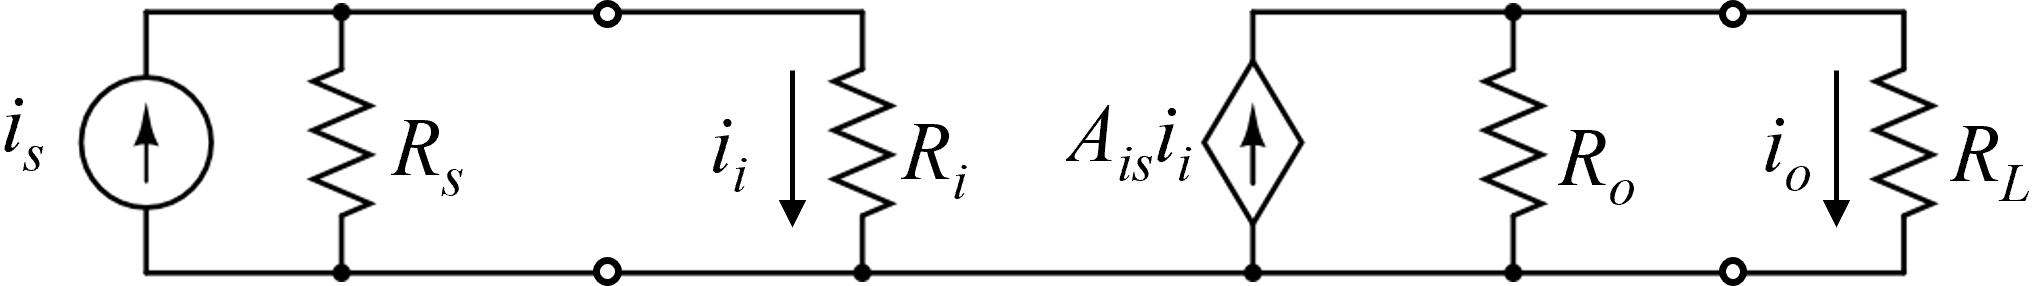
\includegraphics[width=6in]{circuit.png}
\end{center}

You are to design the amplifier according to the following design constraints:

I. The attenuation loss at the amplifier input is at most 17\%.

II. Doubling $R_{L}$ should not change the output current by more than 17\%.

III. The overall current gain is at least 17.

\begin{partquestion}{minshortcircuitgain}{Find the minimum short-circuit current gain $A_{is}$.}
\begin{answer}
    \begin{kaitlyn}
    \noindent\fbox{%
\begin{minipage}{\dimexpr\textwidth-2\fboxsep-2\fboxrule\relax}
            \textbf{Why we're doing this problem:} Nothing is ever really $A_i i_i = i_o.$
            Why? Because the source and load attached to an amplifier (which is how any circuit exists) creates loading effects.
\end{minipage}%
      }%



The goal of this problem is to characterize the amplifier itself. Let's remember what an ideal current amplifier should do:

At the input for a current amplifier, we want as much of the source current as possible to enter the amplifier. Since the source current splits between $R_s$ and $R_i$, we want $R_i \rightarrow 0.$

At the output, the amplifier produces an output current that splits between $R_o$ and $R_L$. We want as much of that current as possible to enter the load, so we want $R_o \rightarrow \infty.$
Thus, an ideal current amplifier has $R_i = 0,$ and $R_o = \infty.$

However, as said in the question, the amplifier is connected to a source with a resistance and a load with its own resistance. These act as a voltage divider and create attenuation at the input and output and prevent our design from acting as the ideal current amplifier above, so we can find what fraction of the source current $i_s$ actually enters the input $i_i$:
\end{kaitlyn} 

    

\[
i_{i} = \frac{R_{s}}{R_{s} + R_{i}} i_{s}
\]

and

\[
i_{o} = \frac{R_{o}}{R_{o} + R_{L}} A_{is} i_{i}
\]

so

\[
A_{i} = \frac{i_{o}}{i_{s}} = \frac{R_{s}}{R_{s} + R_{i}} A_{is} \frac{R_{o}}{R_{o} + R_{L}}.
\]

The first term in this expression is input attenuation due to the current divider, and similarly, the last term is the output attenuation. To satisfy design constraint I, we require:

\begin{align*}
    \frac{R_s}{R_s + R_i} &\geq 0.83 \\
    0.17 R_s &\geq 0.83 R_i \\
    R_i &\leq 0.205R_s
\end{align*}

\begin{kaitlyn}

To satisfy constraint II, we can start from this:

\[i_o =\frac{R_o}{R_o+R_L}A_{is}i_i,\]

and say that increasing $R_L$ changes the output current division. If $R_L$ increases, less current is steered through the load and more remains through $R_o$, so $i_o$ decreases. We therefore compare the new output current with load $2R_L$ to the original output current with load $R_L$:

\[\frac{i_{o,2R_L}}{i_{o,R_L}} \geq 0.83.\]
    
\end{kaitlyn}

which can be simplified to:

\begin{align*}
    R_o + R_L &\geq 0.83R_o + 1.66R_L \\
    0.17 R_o &\geq 0.66 R_L \\
    R_o &\geq 3.88 R_L
\end{align*}

To ensure design constraint III (that the overall current gain meets the minimum value), we choose the worst-case values for the input and output resistances with $R_{i} = 0.205 R_{s}$ and $R_{o} = 3.88 R_{L}$. Plugging these into the expression for overall gain gives:

\begin{align*}
A_i &= \frac{R_s}{R_s + R_i} A_{is} \frac{R_o}{R_o + R_L} \geq 17 \\
&= \frac{R_s}{R_s + 0.205 R_s} A_{is} \frac{3.88 R_L}{3.88 R_L + R_L} \geq 17 \\
&= \frac{1}{1.205}A_{is} \frac{3.88}{4.88} \geq 17 \\
&= 0.660 A_{is} \geq 17
\end{align*}

and it follows that $A_{is,\min} = 25.7$.
\begin{kaitlyn}

\noindent\fbox{%
\begin{minipage}{\dimexpr\textwidth-2\fboxsep-2\fboxrule\relax}
        \textbf{Why this matters:} The amplifier itself must have a short-circuit current gain of at least $A_{is}=25.7$. Even though the desired \emph{overall} current gain is only 17, some of the available gain is lost because not all of the source current enters the amplifier and not all of the amplifier's output current reaches the load. The intrinsic amplifier must therefore provide extra gain to overcome these loading losses.
\end{minipage}%
}

\end{kaitlyn}
\end{answer}
\end{partquestion}

\begin{partquestion}{maxinputres}{If $R_{s} = 100\ \text{k}\Omega$ and $R_{L} = 1\ \text{k}\Omega$, find the maximum $R_{i}$ and the minimum $R_{o}$.}
\begin{answer}
From the results of part (\cref{prob:curramp:minshortcircuitgain}):

\[
R_{i} \leq 0.205 R_{s} = 0.205 \cdot 100\ \text{k}\Omega = 20.5\ \text{k}\Omega,
\]

and

\[
R_{o} \geq 3.88 R_{L} = 3.88 \cdot 1\ \text{k}\Omega = 3.88\ \text{k}\Omega.
\]
\end{answer}
\end{partquestion}

\begin{partquestion}{equivalentvoltagegain}{If this amplifier were to be represented by an equivalent voltage amplifier (with identical values for the three parameters found in parts (\cref{prob:curramp:minshortcircuitgain}) and (\cref{prob:curramp:maxinputres})), what would $A_{vo}$ be?}
\begin{answer}
Since the current amplifier would have an open-circuit output voltage of $A_{is} i_{i} R_{o}$, this must equal that of a standard voltage amplifier with open-circuit output voltage of $A_{vo} v_{i}$. Recall $i_{i} = \frac{v_{i}}{R_{i}}$ so we can write:

\begin{align*}
    A_{vo} v_i &= A_{is} i_{i} R_o \\
    A_{vo} v_i &= A_{is} \frac{v_i}{R_i} R_o \\
    A_{vo} &= A_{is} \frac{R_o}{R_i} \\
    &= 25.7 \frac{3.88}{20.5} \\
    &= 4.86
\end{align*}
\begin{kaitlyn}

\noindent\fbox{%
\begin{minipage}{\dimexpr\textwidth-2\fboxsep-2\fboxrule\relax}
        \textbf{Why this matters:} Remember ideals for a current amplifier:
        \begin{align*}
            R_i << R_s
        \end{align*} and
        \begin{align*}
            R_L << R_o
        \end{align*}

        because we want to design an easy path for all of the source current to enter the amplifier, rather than flow through the source's own impedance. \textbf{Once you connect amplifers to real devices, gain alone isn't the end of story -- we need to design its input and output impedances for the devices it interfaces with.}
\end{minipage}%
}

\end{kaitlyn}
\end{answer}
\end{partquestion}

\end{mainquestion}
